% Options for packages loaded elsewhere
\PassOptionsToPackage{unicode}{hyperref}
\PassOptionsToPackage{hyphens}{url}
%
\documentclass[
]{article}
\usepackage{amsmath,amssymb}
\usepackage{iftex}
\ifPDFTeX
  \usepackage[T1]{fontenc}
  \usepackage[utf8]{inputenc}
  \usepackage{textcomp} % provide euro and other symbols
\else % if luatex or xetex
  \usepackage{unicode-math} % this also loads fontspec
  \defaultfontfeatures{Scale=MatchLowercase}
  \defaultfontfeatures[\rmfamily]{Ligatures=TeX,Scale=1}
\fi
\usepackage{lmodern}
\ifPDFTeX\else
  % xetex/luatex font selection
\fi
% Use upquote if available, for straight quotes in verbatim environments
\IfFileExists{upquote.sty}{\usepackage{upquote}}{}
\IfFileExists{microtype.sty}{% use microtype if available
  \usepackage[]{microtype}
  \UseMicrotypeSet[protrusion]{basicmath} % disable protrusion for tt fonts
}{}
\makeatletter
\@ifundefined{KOMAClassName}{% if non-KOMA class
  \IfFileExists{parskip.sty}{%
    \usepackage{parskip}
  }{% else
    \setlength{\parindent}{0pt}
    \setlength{\parskip}{6pt plus 2pt minus 1pt}}
}{% if KOMA class
  \KOMAoptions{parskip=half}}
\makeatother
\usepackage{xcolor}
\usepackage[margin=1in]{geometry}
\usepackage{graphicx}
\makeatletter
\def\maxwidth{\ifdim\Gin@nat@width>\linewidth\linewidth\else\Gin@nat@width\fi}
\def\maxheight{\ifdim\Gin@nat@height>\textheight\textheight\else\Gin@nat@height\fi}
\makeatother
% Scale images if necessary, so that they will not overflow the page
% margins by default, and it is still possible to overwrite the defaults
% using explicit options in \includegraphics[width, height, ...]{}
\setkeys{Gin}{width=\maxwidth,height=\maxheight,keepaspectratio}
% Set default figure placement to htbp
\makeatletter
\def\fps@figure{htbp}
\makeatother
\setlength{\emergencystretch}{3em} % prevent overfull lines
\providecommand{\tightlist}{%
  \setlength{\itemsep}{0pt}\setlength{\parskip}{0pt}}
\setcounter{secnumdepth}{-\maxdimen} % remove section numbering
\ifLuaTeX
  \usepackage{selnolig}  % disable illegal ligatures
\fi
\usepackage{bookmark}
\IfFileExists{xurl.sty}{\usepackage{xurl}}{} % add URL line breaks if available
\urlstyle{same}
\hypersetup{
  pdftitle={Završni izvještaj: Usporedba programskih alata za procjenu ionosferskog kašnjenja GNSS signala},
  hidelinks,
  pdfcreator={LaTeX via pandoc}}

\title{Završni izvještaj: Usporedba programskih alata za procjenu
ionosferskog kašnjenja GNSS signala}
\author{}
\date{\vspace{-2.5em}2025-06-14}

\begin{document}
\maketitle

\subsection{Osnovne informacije o
projektu}\label{osnovne-informacije-o-projektu}

\begin{itemize}
\tightlist
\item
  \textbf{Naziv projekta:} Usporedba programskih alata za procjenu
  ionosferskog kašnjenja GNSS signala
\item
  \textbf{Studenti:} Antonio Cvitković, Luka Ivanić, Lorena Pekić, Rea
  Prpić
\item
  \textbf{Kodno ime tima:} Tim 8
\item
  \textbf{Profesor:} naslovni prof. dr. sc. Renato Filjar
\item
  \textbf{Ustanova:} Tehnički fakultet u Rijeci
\item
  \textbf{Početak projekta:} 23. svibnja 2025.
\item
  \textbf{Završetak projekta:} 13. lipnja 2025.
\end{itemize}

Projekt se provodi u sklopu nastave kolegija Programski određen radio s
glavnim ciljem dubljeg upoznavanja s programskim okruženjem za
statističko računarstvo R, novim programskim alatima (tec-suite i GPS
TEC), odgovarajućim knjižnicama te samog procesa planiranja i provedbe
projektnog zadatka.

\section{1. Uvod}\label{uvod}

Ukupni sadržaj elektrona u ionosferi (TEC - eng. \emph{Ionospheric Total
Electron Content}) ključni je parametar u razumijevanju dinamike
ionosfere, koji utječe na širenje signala Globalnog navigacijskog
satelitskog sustava (GNSS) i primjene poput navigacije i prognoziranja
svemirskog vremena \hyperref[izvori]{{[}1{]}}. TEC predstavlja broj
slobodnih elektrona duž linije vidljivosti između GNSS prijemnika i
satelita, obično mjeren u TEC jedinicama (TECU,
\(1 , \text{TECU} = 10^{16} , \text{elektrona/m}^2\)). Cilj ovog
projekta je usporediti dva alata, GPS TEC i tec-suite, za procjenu TEC-a
iz GNSS pseudo-udaljenosti, posebno korištenjem GPS podataka iz RINEX
datoteke promatranja \hyperref[izvori]{{[}1{]}{[}2{]}}. Usporedba
uključuje obradu istog skupa podataka s oba alata, izračunavanje
reziduala
(\(r(t) = \text{TEC}{\text{tec-suite}}(t) - \text{TEC}{\text{GPS TEC}}(t)\))
i analizu njihovih statističkih svojstava (kvartili, srednja vrijednost,
varijanca, normalnost) radi procjene točnosti i konzistentnosti.

Skup podataka, dobiven s EarthScope Data Servera, sastoji se od RINEX
datoteke promatranja (ac121600.25o.Z) sa stanice AC12 9. lipnja 2025.
(160. dan) i odgovarajuće GPS navigacijske datoteke (ac121600.25n.Z).
Ciljevi su procijeniti performanse GPS TEC-a i tec-suite-a u smislu
točnosti procjene TEC-a, jednostavnosti korištenja i kompatibilnosti
izlaznih podataka, doprinoseći širem razumijevanju alata za modeliranje
ionosfere. Ovo izvješće detaljno opisuje metodologiju za prikupljanje
podataka i generiranje TEC procjena, s naglaskom na izazove koji se
javljaju pri obradi izlaznih podataka za analizu u R-u.

\section{2. Metodologija}\label{metodologija}

\subsection{Prikupljanje podataka}\label{prikupljanje-podataka}

RINEX datoteka promatranja ac121600.25o.Z preuzeta je s EarthScope Data
Servera
(\url{https://gage-data.earthscope.org/archive/gnss/rinex/obs/2025/160}),
koji pruža GNSS podatke za znanstvena istraživanja
\hyperref[izvori]{{[}3{]}}. Ova komprimirana datoteka, koja se pridržava
RINEX 3.04 formata, sadrži mjerenja pseudo-udaljenosti i faze nosača s
GPS satelita za stanicu AC12 9. lipnja 2025. Odgovarajuće GPS
navigacijske datoteke (ac121600.25n.Z, ac121600.25e.Z, ac121600.25g.Z,
ac121600.25h.Z) također su dobivene iz istog izvora kako bi se osigurale
satelitske efemeride i korekcije sata potrebne za procjenu TEC-a.

\subsection{Korištenje TEC GPS programskog
alata}\label{koriux161tenje-tec-gps-programskog-alata}

Alat GPS TEC, koji je razvio Gopi Seemala, korišten je za obradu RINEX
datoteke promatranja ac121600.25o radi procjene TEC-a. Nakon prilagodbe
postavki radi omogućavanja izlaza datoteka, GPS TEC je generirao jednu
.Cmn datoteku koja sadrži procjene TEC-a sa stupcima: MJdatet, Time,
PRN, Az, Ele, Lat, Lon, Stec, Vtec i S4. Stupac Vtec (vertikalni TEC u
TECU) korišten je za usporedbu, izveden iz mjerenja pseudo-udaljenosti
(P1/P2) nakon izravnavanja nosioca u kod. Datoteka je uključivala dva
retka metapodataka, koji su preskočeni tijekom analize. Na slici 1 vidi
se grafičko sučelje samog programa, te izlaz koji prikaže nakon uspješne
TEC estimacije. Na lijevoj strani je prikazan graf TEC kroz vrijeme od
24h jednog dana, sa korištenim TECU vrijednostima za TEC i sat za
vrijeme. Na desnoj strani je graf TEC (y os) kroz vrijeme (x os) s
uklonjenim satelitskim i prijemnim pristranostima. Na slici 2 prikazan
je prvotni .Cmn izlaz s neobrađenim podacima.

\begin{figure}

{\centering 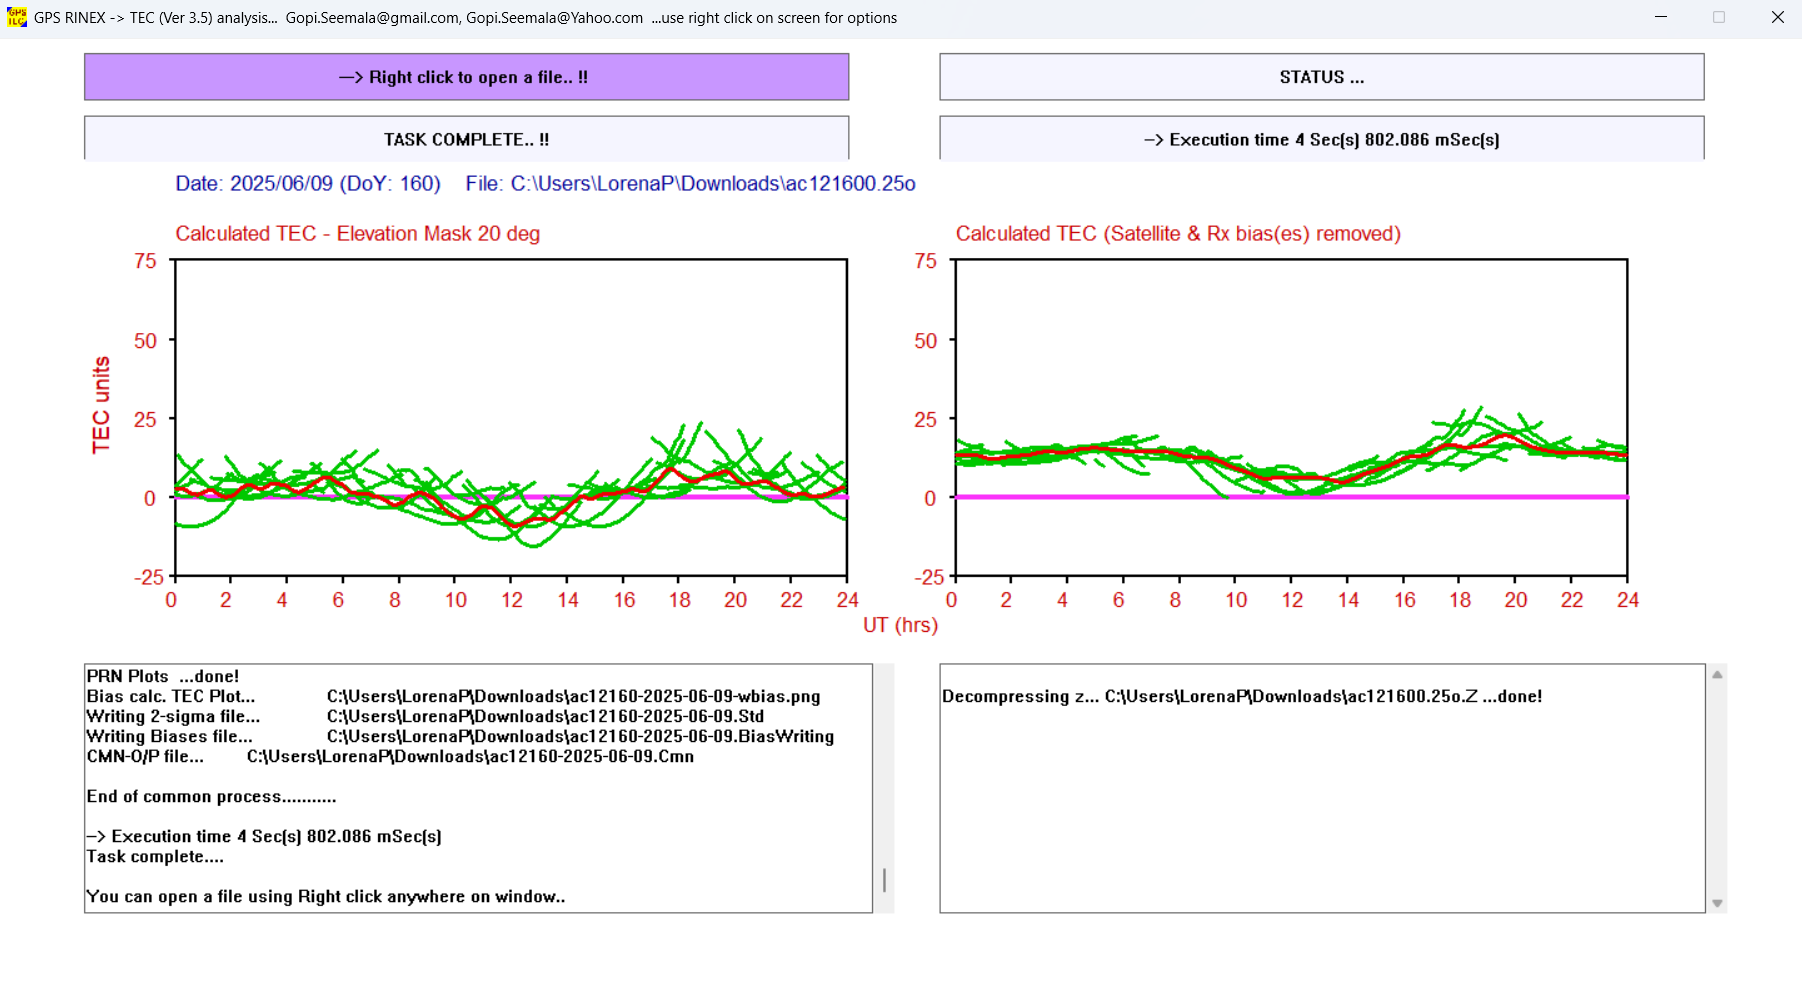
\includegraphics[width=25.03in]{./slike/tecgps-gui} 

}

\caption{**Slika 1:** *Prikaz grafičkog sučelja i izlaza programskog alata TEC GPS*}\label{fig:tecgps-gui}
\end{figure}

\begin{figure}

{\centering 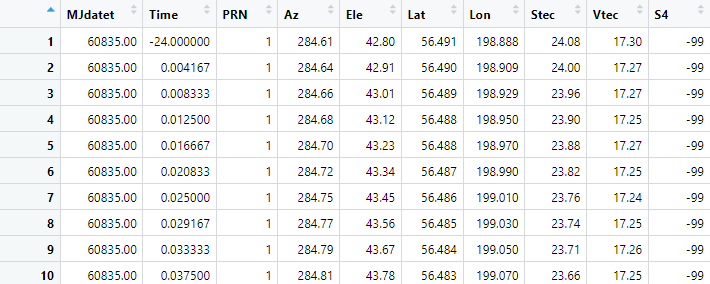
\includegraphics[width=0.7\linewidth]{./slike/tecgps-data} 

}

\caption{**Slika 2:** *Prikaz TEC GPS izlaznih podataka prije obrade*}\label{fig:tecgps-data}
\end{figure}

\subsection{Korištenje tec-suite programskog
alata}\label{koriux161tenje-tec-suite-programskog-alata}

Alat tec-suite korišten je za obradu iste RINEX datoteke (ac121600.25o)
s GPS navigacijskim datotekama (.25n, .25e, .25g i .25h) za generiranje
TEC procjena. Tec-suite nema grafičko sučelje već se sastoji od
direktorija u kojem su izvršna datoteka te konfiguracijska datoteka gdje
se upisuju nazivi direktorija gdje se nalaze potrebne datoteke za
izvršenje programa \hyperref[izvori]{{[}2{]}}. Za ispravan rad programa
potrebno je zasebno instalirati gunzip i crx2rnx koje dekompresiraju
kompaktne RINEX datoteke. Navigacijske datoteke smještene su u zasebne
direktorije (nav/n, nav/g/, nav/h/ i nav/e/ za GLONASS i SBAS) kako bi
se zadovoljili ulazni zahtjevi tec-suitea. Umjesto jedne CSV datoteke,
tec-suite je generirao otprilike 37 .dat datoteka, jednu po vidljivom
GPS satelitu (npr. G01, G02, \ldots, G37). Svaka .dat datoteka imala je
zaglavlje od 10 redaka s metapodacima (npr. PRN satelita, koordinate
lokacije) i stupcima: tsn, sat, el, az, tec.l1l2, tec.p1p2 i valjanost
(eng. \emph{validity}). Stupac tec.p1p2 korišten je kao VTEC za
usporedbu s Vtec-om GPS TEC-a. Zaglavlje je označavalo podatke odvojene
razmacima i format datuma i vremena (\%Y-\%m-\%dT\%H:\%M:\%S), ali retci
podataka koristili su tsn (modificirani julijanski datum) i sat
(decimalni sati). Na slici 3 prikazani su neobrađeni podaci jedne od
.dat datoteke koje je tec-suite izgenerirao.

\begin{figure}

{\centering 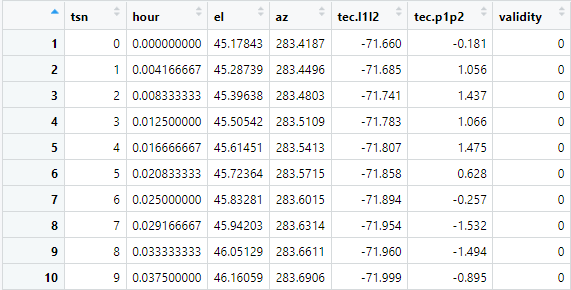
\includegraphics[width=0.7\linewidth]{./slike/tec-suite-data} 

}

\caption{**Slika 3:** *Prikaz tec-suite izlaznih podataka prije obrade*}\label{fig:tesuite_izlaznih_podataka_prije_obrade}
\end{figure}

\section{3. Rezultati}\label{rezultati}

\subsection{Analiza razlike između alata tec-suite i GPS TEC
(Gopi)}\label{analiza-razlike-izmeux111u-alata-tec-suite-i-gps-tec-gopi}

Cilj analize bio je usporediti učinkovitost dvaju programskih alata za
procjenu ukupnog elektronskog sadržaja u ionosferi (TEC):
\emph{tec-suite} i \emph{GPS TEC (Gopi)}. Reziduali su definirani kao
razlika između njihovih procjena u svakom vremenskom trenutku:

\[
r(t) = TEC_{\text{tec-suite}}(t) - TEC_{\text{GPS TEC}}(t)
\]

Gdje TEC označava \emph{Total Electron Content}, odnosno količinu
elektrona po kvadratnom metru između GNSS satelita i prijamnika. Veće
vrijednosti TEC-a ukazuju na gušću ionosferu koja više utječe na
kašnjenje GNSS signala.

Pozitivan rezidual znači da tec-suite precjenjuje količinu elektrona u
odnosu na alat GPS TEC (Gopi), tj. smatra ionosferu gušćom, što može
dovesti do pretjeranih korekcija GNSS signala. Nasuprot tome, negativan
rezidual ukazuje na podcjenjivanje TEC-a od strane tec-suite, što može
rezultirati nedovoljnom korekcijom ionosferskog utjecaja.

Analiza je provedena na podacima istih PRN satelita u istim vremenskim
trenucima, koji su preuzeti s EarthScope Data Servera i i obrađeni
pomoću modela tec-suite i GPS TEC (Gopi). Time svaki izračunati rezidual
precizno prikazuje trenutnu razliku između dvaju modela za isti satelit,
u istom trenutku i pod istim uvjetima.

\subsection{Vremenska dinamika
reziduala}\label{vremenska-dinamika-reziduala}

Analiza vremenskog prikaza reziduala za sve PRN satelite pruža pregled
cjelokupnog ponašanja razlika između alata tec-suite i GPS TEC (Gopi)
kroz promatrano razdoblje. Većina reziduala zadržava se u negativnom
području, što ukazuje na tendenciju alata tec-suite da podcjenjuje
vrijednosti TEC-a u odnosu na referentni alat.

Na grafu su prikazane pojedinačne točke reziduala kroz vrijeme, dok crna
glatka linija vizualizira prosječnu dinamiku odstupanja. Iako ta linija
varira tijekom vremena, jasno se vidi da se zadržava ispod nulte
vrijednosti, što sugerira prevladavajući negativni pomak u procjenama.

Ovaj vremenski pregled ukazuje da performanse alata nisu potpuno
konzistentne kroz cijelo razdoblje, nego pokazuju određene fluktuacije
koje su važne za detaljniju interpretaciju i usporedbu modela. Takva
vremenska varijabilnost stoga predstavlja ključni kontekst za kasniju
statističku analizu po pojedinim PRN satelitima.

\subsection{Gustoća globalnih
reziduala}\label{gustoux107a-globalnih-reziduala}

Analiza ukupne distribucije reziduala između alata tec-suite i GPS TEC
(Gopi) za sve PRN satelite prikazana je histogramom s procijenjenom
funkcijom gustoće vjerojatnosti. Na ovom prikazu jasno je vidljivo da su
gotovo svi reziduali smješteni u negativnom području, što potvrđuje da
tec-suite u velikoj većini slučajeva procjenjuje manji ukupni
elektronski sadržaj (TEC) u odnosu na referentni alat GPS TEC (Gopi).

Najveća gustoća reziduala koncentrirana je u rasponu od otprilike -140
do -50, gdje se pojavljuju dva izražena lokalna maksimuma. Međutim,
gledajući cijeli raspon distribucije, vidljivo je više manjih vrhova.

Najveća učestalost reziduala zabilježena je u rasponu od -140 do -50,
gdje se nalaze dva dominantna vrha. No, gledajući širu raspodjelu,
vidljivo je više manjih lokalnih maksimuma, što znači da razlike među
alatima nisu raspoređene jednoliko. Takav obrazac s više izraženih
područja povećane učestalosti, upućuje na to da razlike između alata
nisu ujednačene, već da postoje tipične razine odstupanja koje se češće
ponavljaju. Te razine mogu biti povezane s određenim PRN satelitima,
vremenskim razdobljima ili promjenjivim ionosferskim uvjetima.

Distribucija nije simetrična ni zvonolikog oblika, već složenija i
razgranatija, s više izraženih gustoća. Ovakva raspodjela pruža dublji
uvid u ponašanje alata i upućuje na to da odstupanja između modela nisu
slučajna, već reflektiraju specifične obrasce i strukturne razlike u
procjenama TEC-a.

\subsection{Globalna deskriptivna
statistika}\label{globalna-deskriptivna-statistika}

Globalni statistički pokazatelji dodatno potvrđuju sustavnu pristranost
modela tec-suite u odnosu na alat GPS TEC (Gopi):

\begin{itemize}
\tightlist
\item
  \textbf{Aritmetička sredina (prosjek)}: −97.4\\
\item
  \textbf{Medijan}: −96.9\\
\item
  \textbf{Minimum / Maksimum}: −217 / 60.2\\
\item
  \textbf{Interkvartilni raspon (IQR)}: 62.1\\
\item
  \textbf{Varijanca}: 1790
\end{itemize}

Ovi pokazatelji jasno potvrđuju da su razlike između alata strukturirane
i konzistentno nagnute prema negativnim vrijednostima. Sredina i medijan
gotovo identične, zajedno s izraženim minimumom, ukazuju na sustavnu
pristranost alata tec-suite. Iako varijanca i IQR upućuju na određenu
razinu varijabilnosti, dominacija negativnih vrijednosti ostaje
najizraženija statistička karakteristika.

\subsection{Statistička analiza reziduala po PRN
satelitima}\label{statistiux10dka-analiza-reziduala-po-prn-satelitima}

Analiza PRN satelita na temelju statističkih pokazatelja
(interkvartilnog raspona (IQR), varijance, položaja medijana i
prisutnosti outliera) omogućila je kategorizaciju njihove pouzdanosti u
kontekstu usporedbe dvaju alata za procjenu totalnog elektronskog
sadržaja (TEC).

Rezultati ukazuju na veliku raznolikost u ponašanju pojedinih PRN
satelita, pri čemu se jasno izdvajaju tri osnovne skupine: pouzdani,
umjereno pouzdani i nestabilni sateliti.

\subsubsection{Visoko pouzdani PRN-ovi}\label{visoko-pouzdani-prn-ovi}

PRN 4, PRN 13, PRN 18, PRN 20 i PRN 22 pokazali su najveći stupanj
stabilnosti i konzistentnosti. Njihove statističke karakteristike --
vrlo uski IQR-ovi, niske varijance te simetrična raspodjela reziduala --
ukazuju na izrazito kompaktne i uravnotežene podatke. Iako PRN 13 i PRN
18 imaju prisutne outliere u pozitivnom smjeru, oni nisu dovoljno
ekstremni da ozbiljno naruše ukupnu stabilnost podataka. PRN 22, iako
ima najveći broj outliera među ovom skupinom, ti su outlieri unutar
prihvatljivih granica i ne narušavaju osnovnu stabilnost. S druge
strane, PRN 4 i PRN 20 gotovo nemaju outliere. U kontekstu usporedbe
dvaju alata, ovi PRN-ovi predstavljaju pouzdanu referencu jer, unatoč
povremenim odstupanjima, ukupno nude visoku preciznost i dosljednost u
procjenama TEC-a.

\subsubsection{Umjereno pouzdani
PRN-ovi}\label{umjereno-pouzdani-prn-ovi}

U ovu kategoriju svrstavaju se PRN 1, 5, 6, 7, 9, 12, 15, 16, 17, 19 i
25. Ovi sateliti pokazali su umjerene razine varijabilnosti, uz
relativno prihvatljive IQR-ove i srednje vrijednosti varijance. U većini
slučajeva prisutni su izolirani outlieri -- najčešće u pozitivnom
smjeru, no bez ozbiljnih posljedica po cjelokupnu raspodjelu. Jezgre
distribucija ostaju relativno stabilne, pa se ovi PRN-ovi mogu smatrati
korektnom osnovom za usporedbu alata, pod uvjetom dodatnog opreza u
tumačenju rezultata.

\subsubsection{Nestabilni i nepouzdani
PRN-ovi}\label{nestabilni-i-nepouzdani-prn-ovi}

PRN 2, 3, 8, 10, 11, 23 i 24 pokazali su široke interkvartilne raspone i
visoke varijance, često uz dodatak izraženih outliera i asimetričnih
distribucija. PRN 10 i PRN 23 posebno su problematični -- s varijancama
od preko 4000 i IQR-ovima većim od 100 jedinica, njihove procjene TEC-a
između alata značajno odstupaju. Ovi PRN-ovi ne mogu se smatrati
pouzdanima za finu procjenu razlika između alata i trebali bi biti
isključeni iz statistički osjetljivih interpretacija.

\subsection{Test normalnosti}\label{test-normalnosti}

Shapiro-Wilk test primijenjen na globalni skup reziduala pokazao je vrlo
niske p-vrijednosti (sve \textless{} 0.05), što jasno upućuje na to da
distribucija reziduala značajno odstupa od normalne. Takav rezultat
potvrđuje nepravilnu i nelinearnu strukturu podataka te opravdava
primjenu statističkih metoda koje ne ovise o pretpostavci normalnosti.
Ova spoznaja dodatno učvršćuje zaključke o neslučajnoj prirodi razlika
između alata i potrebi za robusnijim analitičkim pristupima.

\section{4. Zaključak}\label{zakljuux10dak}

Analiza provedena nad ukupnim skupom reziduala, zajedno s vremenskim
pregledom i pojedinačnom analizom po satelitima, jasno pokazuje da alat
tec-suite dosljedno daje niže vrijednosti TEC-a u odnosu na referentni
alat GPS TEC (Gopi). Takva razlika nije rezultat nasumičnih oscilacija,
već proizlazi iz strukturnih karakteristika modela i njihove različite
osjetljivosti na podatke i uvjete.

Reziduali su u velikoj većini negativni, s izraženim obrascima i
ponavljajućim odstupanjima, što je potvrđeno histogramima gustoće,
deskriptivnom statistikom i testom normalnosti. Distribucija odstupanja
pokazala se nelinearna i nesimetrična, čime se dodatno ističe složenost
razlika između alata. Statistička analiza po PRN satelitima pokazala je
značajne razlike u stabilnosti i preciznosti među satelitima, pri čemu
su neki PRN-ovi iskazali visoku pouzdanost, a drugi visoku varijabilnost
i prisutnost ekstremnih odstupanja.

U cjelini, GPS TEC (Gopi) se ističe kao pouzdaniji i stabilniji alat za
procjenu ukupnog elektronskog sadržaja, s izlaznim vrijednostima koje se
bolje uklapaju u očekivane obrasce i daju manje oscilacija. Za potrebe
budućih analiza, osobito onih koje zahtijevaju visoku preciznost u
modeliranju ionosferskih utjecaja na GNSS signale, preporuča se primjena
Gopi alata kao primarnog izvora TEC procjena.

\section{Izvori}\label{izvori}

\begin{enumerate}
\def\labelenumi{\arabic{enumi}.}
\tightlist
\item
  GPS TEC Program, Seemala Gopi, mrežna stranica:
  \url{https://seemala.blogspot.com/} (pristup: 23.05.2025.)
\item
  tec-suite Documentation, tec-suite Developers, mrežna stranica:
  \url{https://tec-suite.readthedocs.io/en/latest/} (pristup:
  23.05.2025.)
\item
  EarthScope GNSS Data Server, EarthScope Consortium, mrežna stranica:
  \url{https://gage-data.earthscope.org/} (pristup: 23.05.2025.)
\end{enumerate}

\end{document}
